% This template has been tested with LLNCS DOCUMENT CLASS -- version 2.20 (24-JUN-2015)

%"runningheads" enables:
%  - page number on page 2 onwards
%  - title/authors on even/odd pages
%This is good for other readers to enable proper archiving among other papers and pointing to
%content. Even if the title page states the title, when printed and stored in a folder, when
%blindly opening the folder, one could hit not the title page, but an arbitrary page. Therefore,
%it is good to have title printed on the pages, too.
\documentclass[runningheads,a4paper]{llncs}[2015/06/24]

%cmap has to be loaded before any font package (such as cfr-lm)
\usepackage{cmap}
\usepackage[T1]{fontenc}

%https://tex.stackexchange.com/questions/57743/how-to-write-%c3%a4-and-other-umlauts-and-accented-letters-in-bibliography#57745
%for german umlauts
\usepackage[utf8]{inputenc}

\usepackage{graphicx}
\usepackage{amsmath} 

%Even though `american`, `english` and `USenglish` are synonyms for babel package (according to https://tex.stackexchange.com/questions/12775/babel-english-american-usenglish), the llncs document class is prepared to avoid the overriding of certain names (such as "Abstract." -> "Abstract" or "Fig." -> "Figure") when using `english`, but not when using the other 2.
%english has to go last to set it as default language
\usepackage[ngerman,english]{babel}
%Hint by http://tex.stackexchange.com/a/321066/9075 -> enable "= as dashes
\addto\extrasenglish{\languageshorthands{ngerman}\useshorthands{"}}

%better font, similar to the default springer font
%cfr-lm is preferred over lmodern. Reasoning at http://tex.stackexchange.com/a/247543/9075
\usepackage[%
rm={oldstyle=false,proportional=true},%
sf={oldstyle=false,proportional=true},%
tt={oldstyle=false,proportional=true,variable=true},%
qt=false%
]{cfr-lm}
%
%if more space is needed, exchange cfr-lm by mathptmx
%\usepackage{mathptmx}

%for demonstration purposes only
\usepackage[math]{blindtext}

%Sorts the citations in the brackets
%It also allows \cite{refa, refb}. Otherwise, the document does not compile.
%  Error message: "White space in argument"
\usepackage{cite}


%% If you need packages for other papers,
%% START COPYING HERE
%% COPY ALSO cmap and fontenc from lines 10 to 12

%extended enumerate, such as \begin{compactenum}
\usepackage{paralist}

%put figures inside a text
%\usepackage{picins}
%use
%\piccaptioninside
%\piccaption{...}
%\parpic[r]{\includegraphics ...}
%Text...

%for easy quotations: \enquote{text}
\usepackage{csquotes}

%enable margin kerning
\usepackage{microtype}

%tweak \url{...}
\usepackage{url}
%\urlstyle{same}
%improve wrapping of URLs - hint by http://tex.stackexchange.com/a/10419/9075
\makeatletter
\g@addto@macro{\UrlBreaks}{\UrlOrds}
\makeatother
%nicer // - solution by http://tex.stackexchange.com/a/98470/9075
%DO NOT ACTIVATE -> prevents line breaks
%\makeatletter
%\def\Url@twoslashes{\mathchar`\/\@ifnextchar/{\kern-.2em}{}}
%\g@addto@macro\UrlSpecials{\do\/{\Url@twoslashes}}
%\makeatother

%diagonal lines in a table - http://tex.stackexchange.com/questions/17745/diagonal-lines-in-table-cell
%slashbox is not available in texlive (due to licensing) and also gives bad results. This, we use diagbox
%\usepackage{diagbox}

%required for pdfcomment later
\usepackage{xcolor}


%enable nice comments
%this also loads hyperref
\usepackage{pdfcomment}
%enable hyperref without colors and without bookmarks
\hypersetup{hidelinks,
   colorlinks=true,
   allcolors=black,
   pdfstartview=Fit,
   breaklinks=true}
%enables correct jumping to figures when referencing
\usepackage[all]{hypcap}

\newcommand{\commentontext}[2]{\colorbox{yellow!60}{#1}\pdfcomment[color={0.234 0.867 0.211},hoffset=-6pt,voffset=10pt,opacity=0.5]{#2}}
\newcommand{\commentatside}[1]{\pdfcomment[color={0.045 0.278 0.643},icon=Note]{#1}}

%compatibality with packages todo, easy-todo, todonotes
\newcommand{\todo}[1]{\commentatside{#1}}
%compatiblity with package fixmetodonotes
\newcommand{\TODO}[1]{\commentatside{#1}}

%enable \cref{...} and \Cref{...} instead of \ref: Type of reference included in the link
\usepackage[capitalise,nameinlink]{cleveref}
%Nice formats for \cref
\crefname{section}{Sect.}{Sect.}
\Crefname{section}{Section}{Sections}

\usepackage{xspace}
%\newcommand{\eg}{e.\,g.\xspace}
%\newcommand{\ie}{i.\,e.\xspace}
\newcommand{\eg}{e.\,g.,\ }
\newcommand{\ie}{i.\,e.,\ }

%introduce \powerset - hint by http://matheplanet.com/matheplanet/nuke/html/viewtopic.php?topic=136492&post_id=997377
\DeclareFontFamily{U}{MnSymbolC}{}
\DeclareSymbolFont{MnSyC}{U}{MnSymbolC}{m}{n}
\DeclareFontShape{U}{MnSymbolC}{m}{n}{
    <-6>  MnSymbolC5
   <6-7>  MnSymbolC6
   <7-8>  MnSymbolC7
   <8-9>  MnSymbolC8
   <9-10> MnSymbolC9
  <10-12> MnSymbolC10
  <12->   MnSymbolC12%
}{}
\DeclareMathSymbol{\powerset}{\mathord}{MnSyC}{180}

% correct bad hyphenation here
\hyphenation{op-tical net-works semi-conduc-tor}

%% END COPYING HERE

\usepackage{subfigure}


\begin{document}

\title{Bilderkennung mit Convolutional Neural Networks}
%If Title is too long, use \titlerunning
%\titlerunning{Short Title}

%Single insitute
\author{Ivo Tremel \and Lennard Nöhren}
%If there are too many authors, use \authorrunning
%\authorrunning{First Author et al.}
\institute{Computational Health Informatics\\ Leibniz Universität Hannover}

%Multiple insitutes
%Currently disabled
%
\iffalse
%Multiple institutes are typeset as follows:
\author{Firstname Lastname\inst{1} \and Firstname Lastname\inst{2} }
%If there are too many authors, use \authorrunning
%\authorrunning{First Author et al.}

\institute{
Insitute 1\\
\email{...}\and
Insitute 2\\
\email{...}
}
\fi
			
\maketitle

\begin{abstract}
Wir haben ein aufs Wesentliche reduziertes Convolutional Netz zur Klassifizierung von je 100  verschiedenen, handschriftlichen Buchstaben des deutschen Alphabets mit Umlauten
in zehn verschiedene Kategorien trainiert. Dabei wurde eine Genauigkeit von 85\% erreicht. Das Convolutional Neural Network (CNN) besteht aus einer Faltungsebene, die von einer Max-Pooling Ebene und einer Fully-Connected Ebene gefolgt wird. Zudem wurde die Erweiterung der Inception-Layers verwendet, welches die Genauigkeit nicht erhöhte.
\end{abstract}

%\begin{keywords}
%keyword1, keyword2
%\end{keywords}

%%%%%%%%%%%%%%%%%%%%%%%%%%%%%%%%%%%%%%%%%%%%%%%%%%%%%%%%%%%%%%%%%%%%%%%%%%%%%%%
\section{Einleitung}\label{sec:intro}
%%%%%%%%%%%%%%%%%%%%%%%%%%%%%%%%%%%%%%%%%%%%%%%%%%%%%%%%%%%%%%%%%%%%%%%%%%%%%%%
%Convolutional Neural Networks kommen nahe an menschliche Leistungen heran und der Ansatz der Faltungsnetze bewahrt die entscheidende Lokalität der Bildinformationen. Allerdings
Deep Learning ist ein aktueller Trend im Bereich des Machine Learnings. Durch architektonische Verbesserungen sowie neue Ansätze zum Training der neuronalen Netze können mehrere Layers und damit versteckte Neuronen genutzt werden. Durch das Hintereinanderschalten von mehreren Layers verbunden mit der nichtlinearen Kombination der jeweiligen Outputs wird eine Projektion des Eingaberaums auf eine niedrigere Dimension erreicht. Jede dieser niedrig dimensionalen Projektionen entspricht dabei einer höher wahrnehmbaren Ebene. Wenn die Gewichte des Netzwerks optimal sind, resultiert das in einer hohen Abstraktionsebene der Daten oder auch z.B. Bilder. Diese Abstraktionsebenen erbringen eine effektive Leistung, weil sie ein automatisches Featureset liefern. Dieses hätte sonst manuell erstellt werden müssen. Unter den verschiedenen methodischen Varianten des Deep Learnings stechen einige besonders hervor. Insbesondere Convolutional Neural Networks (CNNs) sind besonders populär. Ihre Architektur lässt sich als eine Menge von hintereinandergeschalteten Layers, bestehend aus den Convolutional Filtern und den darauf folgenden Pooling Layers, beschreiben. Jedes Layer des Netzwerks bringt dabei ein abstraktes Feature hervor. Diese biologisch inspirierte Architektur ähnelt den Abläufen, in denen der visuelle Cortex bildliche Informationen über rezeptive Felder aufnimmt \cite{ravi}.

Das Erkennen von handschriftlichen Texten in Echtzeit ist eine Funktion, die in vielen Bereichen genutzt werden könnte. Allerdings muss man dafür eine präzise Bildanalyse durchführen, was im Allgemeinen einen hohen Rechenaufwand mit sich bringt. In den letzten Jahren hat der sehr schnelle Fortschritt in dem Bereich Machine Learning und insbesondere Neuronale Netze allerdings eine gute Lösung für diese Problematik hervorgebracht. CNNs haben großartige Ergebnisse bei allen möglichen Arten der Bildanalyse gezeigt und sind auch ausgezeichnet zum Erkennen von Buchstaben geeignet. Es werden auch immer wieder neue Verbesserungen für CNN's entwickelt, welche die Präzision der Klassifizierung und die Laufzeit stetig verbessern. Eine dieser Erweiterungen sind die so genannten Inception Module, welche im Jahr 2014 das erste mal in GoogLeNet verwendet wurden \cite{inception_paper}. Das dort beschriebene Netz hat den ersten Platz im ILSVRC(ImageNet Large Scale Visual Recognition Competition) 2014 belegt.\\
Im folgenden wird ein klassisches CNN und ein CNN mit einem Inception Modul für eine Zeichenerkennung genutzt und die Performance der beiden Netze wird verglichen.\\

\section{Datensatz}\label{sec:dataset}
Der genutzte Datensatz besteht aus 1000 handschriftlichen Buchstaben des deutschen Alphabets, die in 10 Klassen klassifiziert werden können. 
\begin{figure}
	%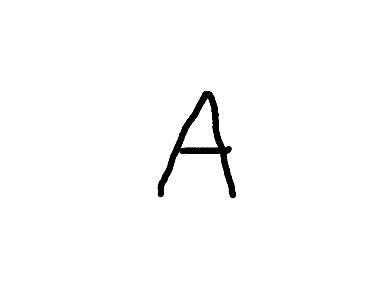
\includegraphics[width=0.2\textwidth]{hand_images/image_Ae_up_106_point_24.png}
	\subfigure{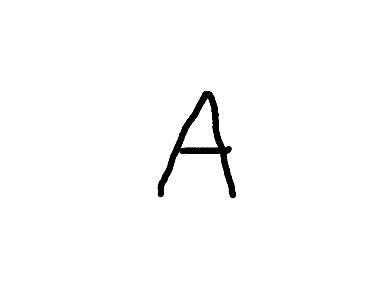
\includegraphics[width=0.2\textwidth]{hand_images/image_Ae_up_106_point_24.png}}
	\subfigure{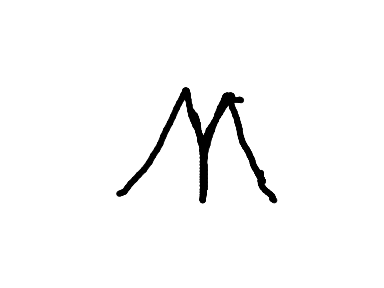
\includegraphics[width=0.2\textwidth]{hand_images/image_M_up_9_point_94.png}}
	\subfigure{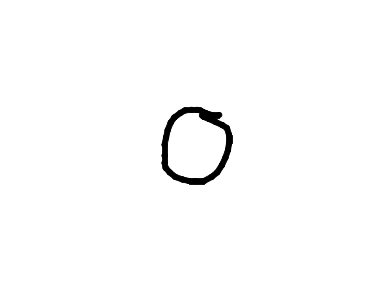
\includegraphics[width=0.2\textwidth]{hand_images/image_O_up_5_point_14.png}}
	\subfigure{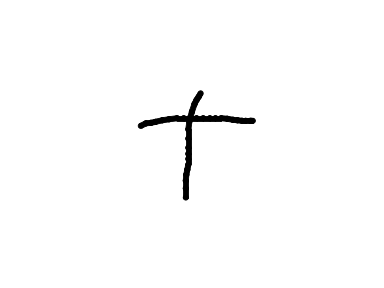
\includegraphics[width=0.2\textwidth]{hand_images/image_T_up_29_point_14.png}}
	\subfigure{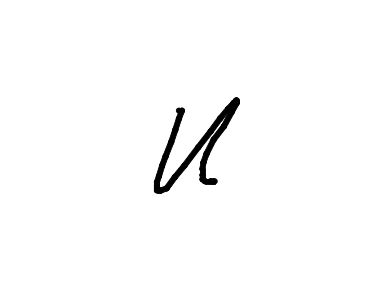
\includegraphics[width=0.2\textwidth]{hand_images/image_U_up_31_point_328.png}}
	\subfigure{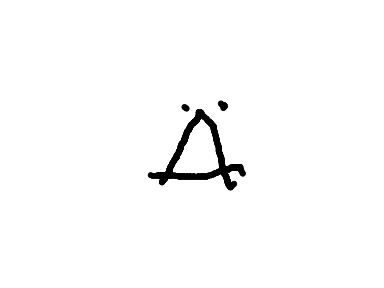
\includegraphics[width=0.2\textwidth]{hand_images/image_Ae_up_142_point_31.png}}
	\subfigure{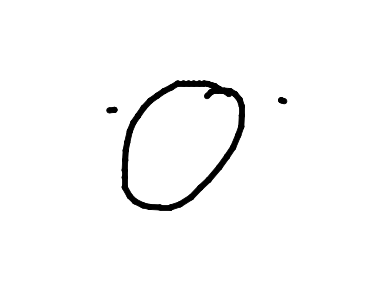
\includegraphics[width=0.2\textwidth]{hand_images/image_Oe_up_157_point_17.png}}
	\subfigure{
\includegraphics[width=0.2\textwidth]{hand_images/image_Ue_up_132_point_13.png}}
	\subfigure{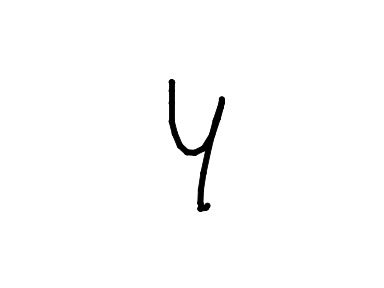
\includegraphics[width=0.2\textwidth]{hand_images/image_Y_up_46_point_8.png}}
	\subfigure{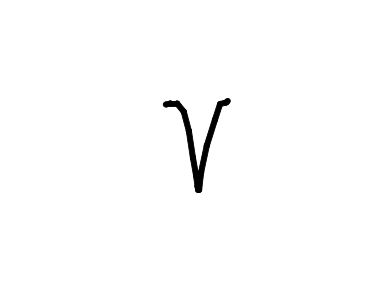
\includegraphics[width=0.2\textwidth]{hand_images/image_V_up_46_point_314.png}}	
	\caption{Beispiele für Buchstaben aus dem Datensatz}
	\label{fig:charexample}
\end{figure}
Die Klassen bestehen aus den Buchstaben A,M,O,T,U und Ä,Ö,Ü,Y,V, die von Kindern geschrieben wurden. In \cref{fig:charexample} sind einige stellvertretende Beispielbuchstaben aus den verschiedenen Klassen zu sehen.
%und auch die schwer unterscheidbaren Umlaute Ä,Ö,Ü,Y,V sind dabei.
Dabei enthält das Datenset die deutschen Umlaute \"{A}, \"{O} und \"{U} als zusätzliche Erschwerung, welche nur besonders schwer von den Buchstaben A, O und U zu unterscheiden sind.

Allerdings mussten wir feststellen, dass einige Labels falsch sind. Bei dem Bild \glqq image\_Ä\_up\_106\_point\_24.png\grqq   ist in \cref{fig:wrongchar} zum Beispiel kein Ä, sondern ein A zu erkennen.

\begin{figure}
	\centering
	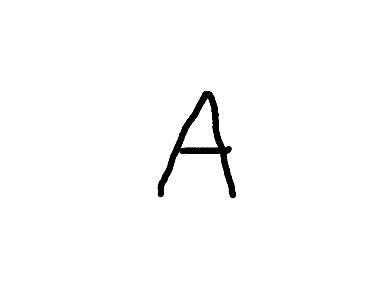
\includegraphics[width=0.2\textwidth]{hand_images/image_Ae_up_106_point_24.png}
	
	\caption{Beispiel für falsch gelabelten Buchstaben}
	\label{fig:wrongchar}
\end{figure}

\section{Materialien und Methoden}\label{sec:material}

\subsection{Klassische Convolutional Neural Networks}
CNNs sind für die Verarbeitung von Daten, die aus mehreren Arrays bestehen, konstruiert. Dies ist zum Beispiel bei einem Farbbild, welches aus drei 2D Arrays besteht, der Fall. In den Arrays des Farbbildes stehen dabei die Pixel Intensitäten der Farbkanäle. Es gibt vier zentrale Ideen bei CNNs, die die Eigenschaften von natürlichen Signalen ausnutzen. Dazu gehören die lokalen Verbindungen, die geteilten Gewichte, das Pooling und die Nutzung von vielen Layers \cite{lecun_nature}. In Bilddaten korrelieren lokale Gruppen von Daten oft sehr stark und bilden damit unterscheidbare lokale Motive, die leicht erkennbar sind. Die Rolle der Convolutional Layers ist die Entdeckung von lokalen Features des vorherigen Layers. Die Pooling Layers haben die Aufgabe semantisch gleiche Features in eins zusammenzuführen.

Bei der Nutzung von tiefen neuronalen Netzen wird die Eigenschaft ausgenutzt, dass viele natürliche Signale aus zusammengesetzten Hierarchien bestehen. Bei Bildern werden aus lokalen Kombinationen von Kanten Motive geformt. Diese können wiederum zu Objekten zusammengeführt werden. Die Convolutional und Pooling Layers in CNNs sind direkt durch die Abläufe von einfachen und komplexen Zellen der visuellen Neurowissenschaft inspiriert. Die gesamte Architektur hat Parallelitäten zu der Hierarchie des visuellen Cortex. 

\subsubsection*{Convolutional Layers:}
Die Neuronen im Convolutional Layer führen eine diskrete Faltung auf dem Eingabebild durch. Dafür verwenden sie eine kleine Matrix, zum Beispiel mit der Größe 5x5, mit der sie über das Bild laufen und jeweils durch das innere Produkt der Matrix die Werte berechnen. Diese Matrix wird Fitlerkernel genannt. Danach wird wie bei normalen Neuronen mithilfe einer Aktivierungsfunktion der Output des Neurons bestimmt. Der Vorteil dieser Methode ist, dass durch den Filterkernel nicht nur einzelne Punkte eines Bildes betrachtet werden, sondern auch die lokale Umgebung von jedem Punkt. Dadurch können größere Features, die aus mehreren Punkten bestehen besser erkannt werden.

\subsubsection*{Pooling Layers:}
In CNNs fassen Pooling-Layers den Output von den vorhergehenden Neuronen entsprechend der gewählten Kernelgröße zusammen. Dabei wird bei einem 2x2 Kernel der größte Output durchgeschaltet und die anderen drei Ausgänge verworfen. Damit wird eine Reduktion der Datenmenge erreicht, die eine insgesamt schnellere Berechnung ermöglicht.

\subsubsection*{Aufbau:}
\begin{figure}
	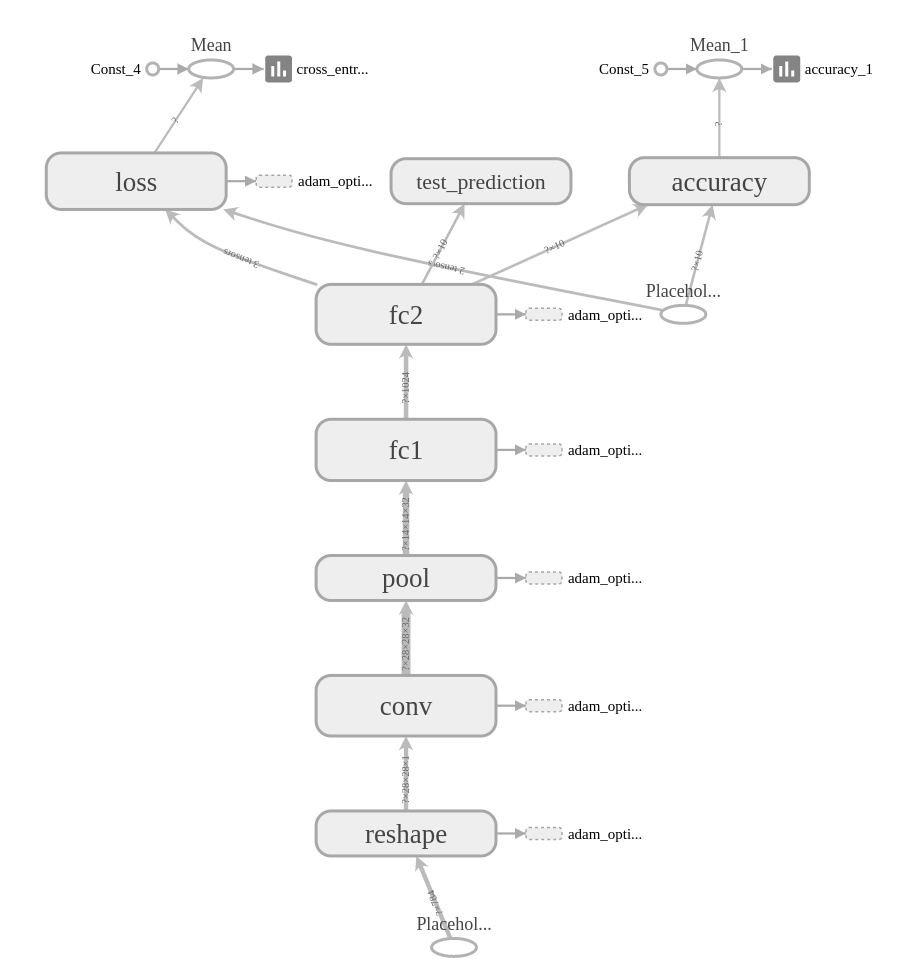
\includegraphics[width=\textwidth]{images/main_graph_conv.png}
	\caption{Main Graph of Classic CNN}
	\label{fig:main_graph_conv}
\end{figure}
\Cref{fig:main_graph_conv} zeigt den Aufbau des CNNs. Vor dem ersten Convolutional Layer wird das Eingabebild zu einem 28x28x1 Bild ("reshape") transformiert. Die erste und zweite Dimension stehen dabei für die Bildhöhe und Bildbreite. Die dritte Dimension bezeichnet die Anzahl von Farbkanälen. Da es sich um ein Graustufenbild handelt und nicht RGB wird der Wert 1 angenommen. 
Bei der Convolution ("conv") werden mit einer Kernelgröße von 5x5 32 Features erzeugt. Danach wird ein Max-Pooling ("pool") mit einer Kernelgröße von 2x2 und einer Schrittweite von 2 durchgeführt. Dadurch wird die Größe des Bildes auf 14x14 reduziert. Anschließend werden die Features in ein Fully-Connected Layer ("fc1") weitergeleitet. Dort werden die Daten in 1024 Nodes verarbeitet und danach an das Output Layer, welches ein Fully-Connected Layer ("fc2")mit 10 Outputs ist, übergeben. Jeder Output steht dabei für einen Buchstaben.

\subsection{CNN mit Inception Layer}
\subsubsection*{Inception Layers:}
\begin{figure}
	\centering
	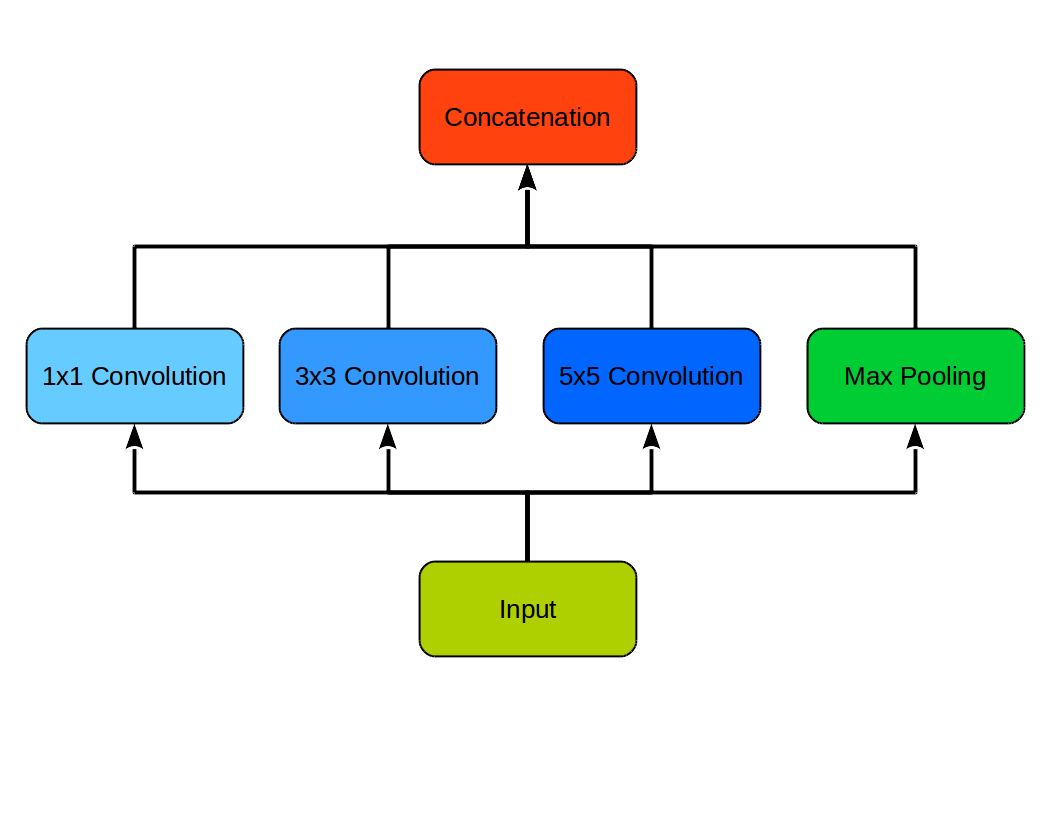
\includegraphics[width=0.9\textwidth]{images/inception_naive_graph.png}
%	\subfigure[Verbesserter Aufbau]{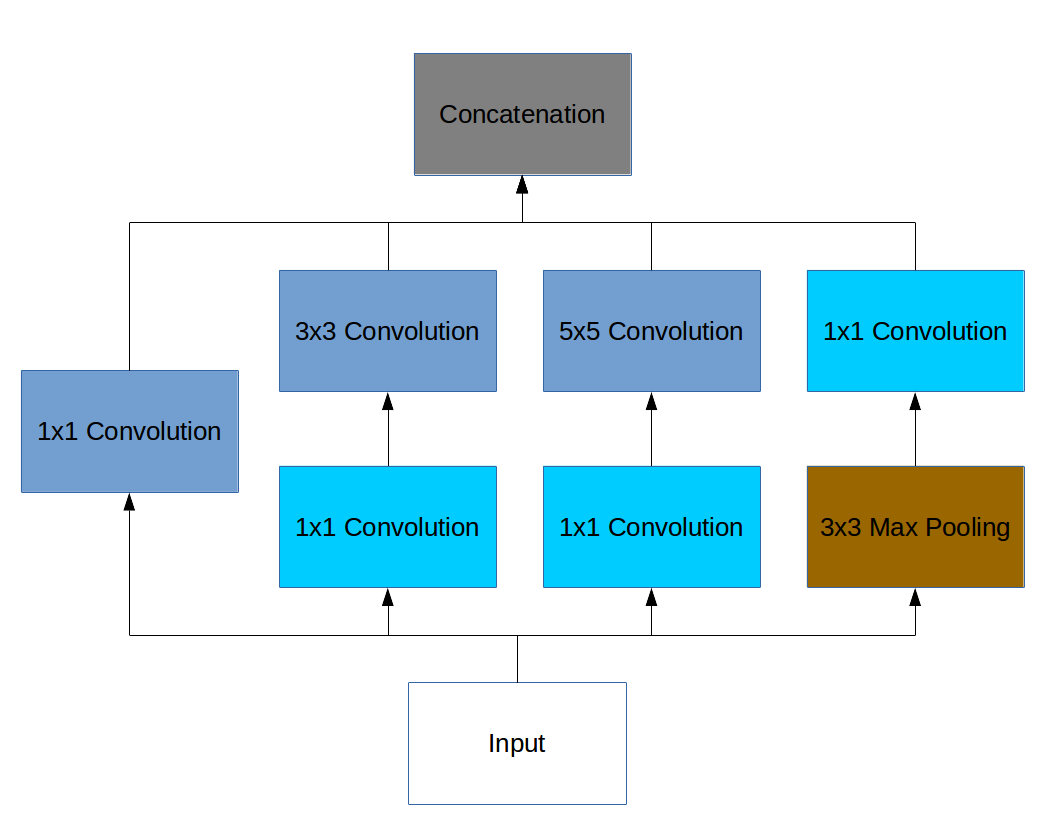
\includegraphics[width=0.49\textwidth]{images/inception_pro_graph.png}}
	\caption{Naiver Aufbau}
	\label{fig:inception_graph}
\end{figure}
\begin{figure}
	%\subfigure[Naiver Aufbau]{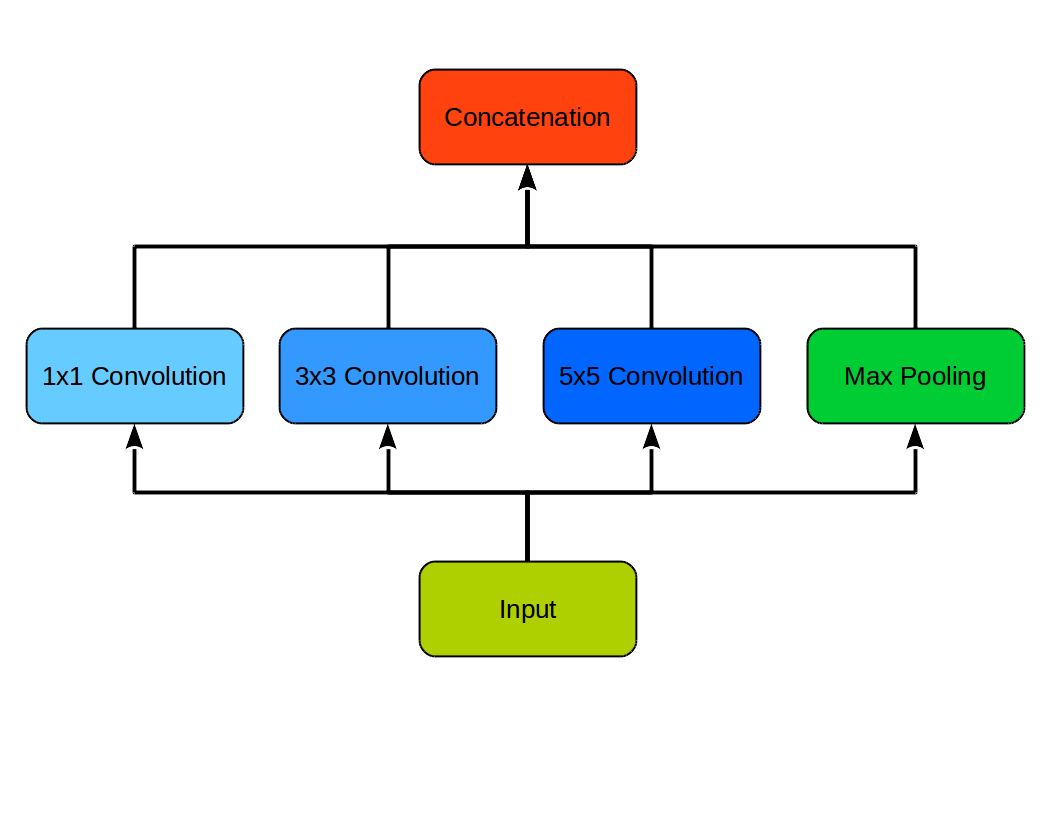
\includegraphics[width=0.49\textwidth]{images/inception_naive_graph.png}}
	\centering
	\subfigure{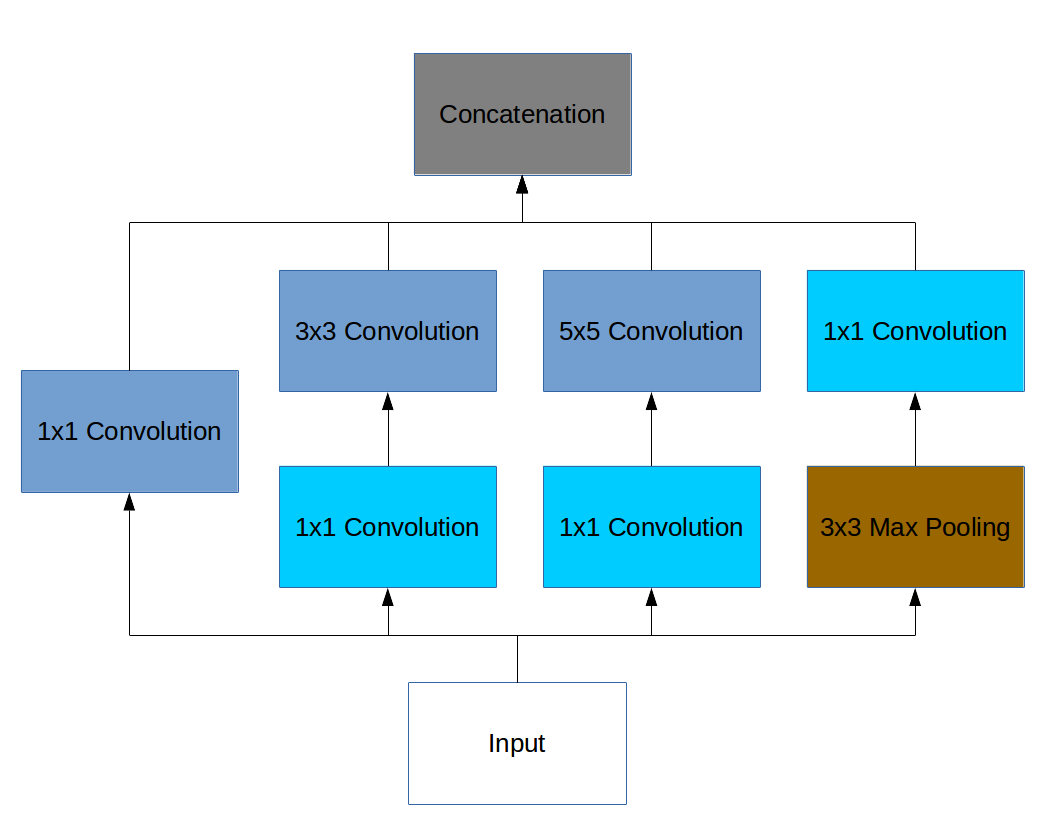
\includegraphics[width=0.9\textwidth]{images/inception_pro_graph.png}}
	\caption{Verbesserter Aufbau}
	\label{fig:inception_graph_improved}
\end{figure}
In einem normalen Convolutional Layer muss festgelegt werden welche Größe der Filterkernel haben soll. Verschieden Größen bringen dabei immer Vor- und Nachteile mit sich. Deshalb ist die Idee von Inception Layers diese Wahl flexibler zu machen und dem Netz zu überlassen. Außerdem wurde in \cite{sparse_paper} gezeigt, das es Vorteile bringt spärlich vernetzte Convolutional Layers zu nutzen. Das ist mit der modernen Rechnerarchitektur allerdings nicht sehr Effizient möglich. Mit Inception Modulen wird versucht diese Eigenschaft anzunähern und trotzdem die aktuelle Hardware maximal auszunutzen.\\
Um das zu ermöglichen enthält ein Inception Layer Convolution Module mit verschiedenen Kernelgrößen und auch Pooling Module, die konkateniert werden. Folgende Motivationen stehen hinter der Nutzung der jeweiligen Module: In den Schichten des Netzes, welche nah am Input sind, macht es mehr Sinn kleinere Features verstärkt zu suchen, wozu 1x1 Convolutions gut geeignet sind. Allerdings wird es auch einige Features geben, die räumlich weit voneinander entfernt sind, weshalb man größere Filter benötigt. Deswegen nutzt man auch 3x3 und 5x5 Convolutions. In den höheren Schichten des Netzes sollten diese verstärkt genutzt werden, um mehr größere Features zu extrahieren. Außerdem haben sich Pooling Layers als sehr wichtig in CNNs erwiesen, weshalb zusätzlich zu den Convolution Modulen auch ein Pooling Modul als alternativer Pfad in das Inception Layer eingefügt wird.\\
In \Cref{fig:inception_graph} und \cref{fig:inception_graph_improved} sieht man nun den Aufbau eines Inception Layers. \cref{fig:inception_graph} zeigt zunächst den Naive Aufbau, wobei alle Module direkt auf den Input angewendet und dann konkateniert werden. Das Problem bei diesem Ansatz ist allerdings, das dieses Layer einen extrem hohen Rechenaufwand hätte und wenn man mehrere Inception Layers hintereinander schalten würde, würde die Größe des Outputs durch die Konkatenation der Outputs der inneren Module immer weiter ansteigen.
Um diese Probleme ein wenig abzuschwächen führt man üblicherweise vor den großen Convolutions jeweils auch eine 1x1 Convolution durch. Dadurch reduziert man die Dimension des Inputs für die großen Module, was zu einer deutlich besseren Laufzeit führt. Dies liefert den Aufbau, den man in \cref{fig:inception_graph_improved} sieht.\\
Die Vorteile dieser Art der Layers in einem CNN gegenüber einem normalen Convolutional Layer sind zum einen, das man durch die Dimensions-Reduktion mehr Operationen durchführen kann, ohne die Laufzeit zu extrem zu steigern. Außerdem ist es sinnvoll visuelle Informationen in verschiedenen Skalierungen zu analysieren, um sowohl große als auch kleine Strukturen erkennen zu können. Dies ist in Inception Modulen in einem Schritt möglich.\\
In großen Inception Netzwerken würde man mehrere dieser Inception Layers hintereinander anwenden und manchmal ein Pooling Layer mit einer Schrittgröße von 2 dazwischen schalten, um die Auflösung zu halbieren, damit der Speicherverbrauch reduziert wird. In \cite{inception_paper} hat sich gezeigt, dass es sinnvoll sein kann Inception Module erst in höheren Layers des Netzes zu nutzen und in den niedrigeren Schichten auf die klassische Architektur von Convolutional Netzen zurückzugreifen.

\subsubsection*{Aufbau:}
\begin{figure}
	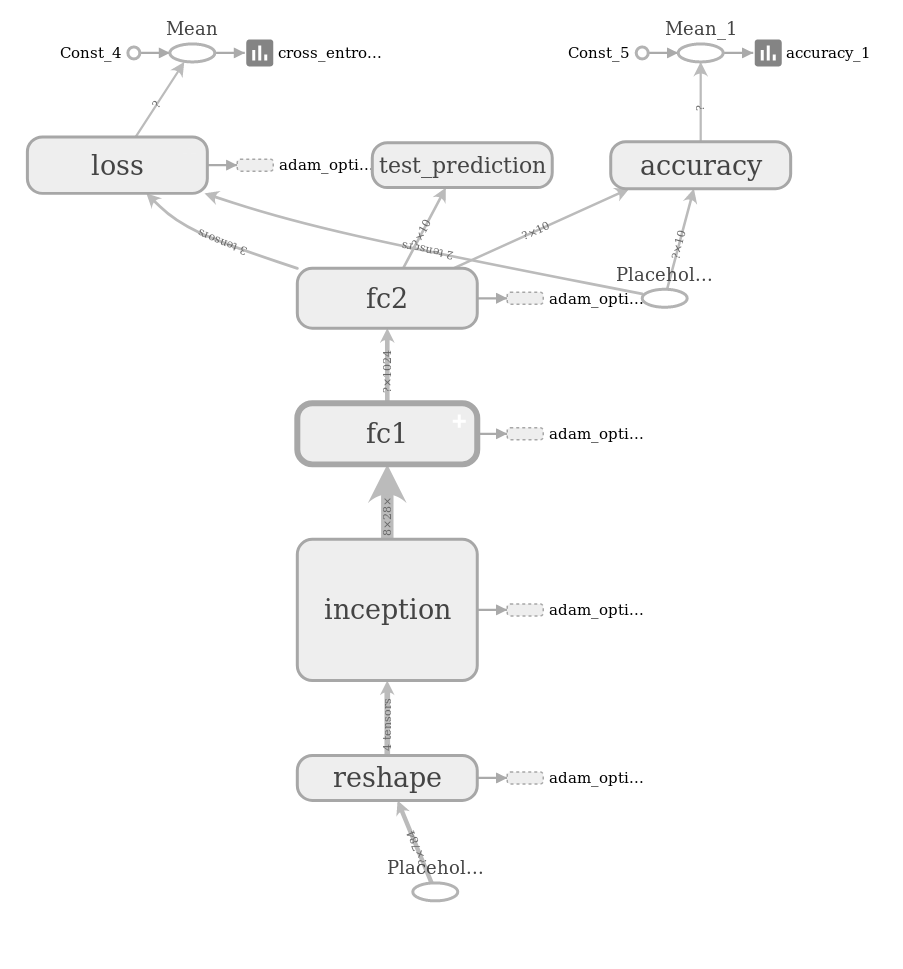
\includegraphics[width=\textwidth]{images/main_graph_inception.png}
	\caption{Main Graph of Inception CNN}
	\label{fig:main_graph_inception}
\end{figure}
\Cref{fig:main_graph_inception} zeigt nun den Aufbau eines Netzes in dem das Convolutional Layer und pooling Layer durch ein Inception Layer ("inception") ersetzt wurde. Dieses bekommt den gleichen Input wie das Convolution Layer im vorher beschriebenen Netz. Der Output des Inception Layers sind 4*32 features. Jedes der 4 Module des Inception Layers erzeugt 32 Features der Größe 28x28, welche dann konkateniert werden. Diese Features werden dann wie vorher durch zwei Fully-Connected Layers ("fc1") und ("fc2") weiter verarbeitet.

\section{Details zu den Lernparametern}
Wir haben unser Model mit Hilfe des AdamOptimizers und einer Batchsize von 50 Beispielen lernen lassen. Die Gewichte in jeder Layer wurden mit einer Gaußverteilung, die den Mittelwert 0 und eine Standardabweichung von 0.1 hat, ermittelt. Zusätzlich wurden Werte, deren Höhe mehr als zwei Standardabweichungen vom Mittelwert abweicht, nicht genommen, sondern erneut zufällig ausgewählt \cite{tensorflow}. Der Neuroneneinfluss (neuron bias) wurde in allen Layers am Anfang auf den Wert 0.1 gesetzt. Die Lernrate hatte das gesamte Training über den Wert 0.0001. Das CNN wurde für 1000 Zyklen mit den 750 Trainingsbildern trainiert. Dies dauerte 5 Minuten, während es bei dem Convolutional Netz mit Inception Layers etwa 30 Minuten dauerte. 

In \cref{fig:kernel} sind die Filter Kernel des ersten Convolutional Layers zu sehen, welche aus den 28x28x1 großen Eingabebildern gelernt wurden. Hohe Werte sind dabei rötlich dargestellt, niedrige positive Werte gelb, negative Werte hingegen sind bläulich. Werte die nahe bei 0 sind, werden grün dargestellt. Die gelernten Gewichte des Convolutional Kernels stellen abstrakte, high-level Features dar, die das CNN gelernt hat. Der 26. Convolutional Kernel erinnert dabei an den horizontal gespiegelten Sobelfilter $G_y$ aus \cref{fig:sobel}. Damit hätte das CNN sich selbst beigebracht horizontale Kanten zu erkennen, um die Buchstaben klassifizieren zu können. Die anderen gelernten Convolutional Kernels könnten andere aus der Bilderkennung bekannte Filter darstellen. Mit diesen könnte das CNN die Eingabebilder nach der Filterung aus einer höheren Abstraktionsebene heraus beurteilen.
\begin{figure}
	\subfigure{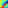
\includegraphics[width=0.1\textwidth]{wl0.pdf}}
	\subfigure{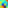
\includegraphics[width=0.1\textwidth]{wl1.pdf}}
	\subfigure{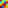
\includegraphics[width=0.1\textwidth]{wl2.pdf}}
	\subfigure{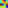
\includegraphics[width=0.1\textwidth]{wl3.pdf}}
	\subfigure{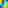
\includegraphics[width=0.1\textwidth]{wl4.pdf}}
	\subfigure{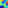
\includegraphics[width=0.1\textwidth]{wl5.pdf}}
	\subfigure{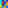
\includegraphics[width=0.1\textwidth]{wl6.pdf}}
	\subfigure{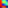
\includegraphics[width=0.1\textwidth]{wl7.pdf}}
	\subfigure{
\includegraphics[width=0.1\textwidth]{wl8.pdf}}
	\subfigure{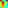
\includegraphics[width=0.1\textwidth]{wl9.pdf}}
	\subfigure{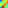
\includegraphics[width=0.1\textwidth]{wl10.pdf}}
	\subfigure{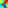
\includegraphics[width=0.1\textwidth]{wl11.pdf}}
	\subfigure{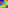
\includegraphics[width=0.1\textwidth]{wl12.pdf}}
	\subfigure{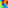
\includegraphics[width=0.1\textwidth]{wl13.pdf}}
	\subfigure{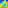
\includegraphics[width=0.1\textwidth]{wl14.pdf}}
	\subfigure{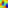
\includegraphics[width=0.1\textwidth]{wl15.pdf}}
	\subfigure{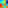
\includegraphics[width=0.1\textwidth]{wl16.pdf}}
	\subfigure{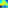
\includegraphics[width=0.1\textwidth]{wl17.pdf}}
	\subfigure{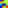
\includegraphics[width=0.1\textwidth]{wl18.pdf}}
	\subfigure{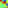
\includegraphics[width=0.1\textwidth]{wl19.pdf}}
	\subfigure{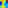
\includegraphics[width=0.1\textwidth]{wl20.pdf}}
	\subfigure{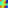
\includegraphics[width=0.1\textwidth]{wl21.pdf}}
	\subfigure{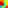
\includegraphics[width=0.1\textwidth]{wl22.pdf}}
	\subfigure{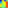
\includegraphics[width=0.1\textwidth]{wl23.pdf}}
	\subfigure{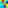
\includegraphics[width=0.1\textwidth]{wl24.pdf}}
	\subfigure{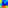
\includegraphics[width=0.1\textwidth]{wl25.pdf}}
	\subfigure{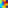
\includegraphics[width=0.1\textwidth]{wl26.pdf}}
	\subfigure{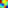
\includegraphics[width=0.1\textwidth]{wl27.pdf}}
	\subfigure{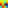
\includegraphics[width=0.1\textwidth]{wl28.pdf}}
	\subfigure{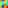
\includegraphics[width=0.1\textwidth]{wl29.pdf}}
	\subfigure{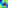
\includegraphics[width=0.1\textwidth]{wl30.pdf}}
	\subfigure{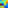
\includegraphics[width=0.1\textwidth]{wl31.pdf}}
	\caption{32 vom ersten Convolutional Layer gelernte Convolution Kernels der Größe 5x5x3}
	\label{fig:kernel}
\end{figure}

Zum Vergleich lassen sich die in der digitalen Bildverarbeitung üblichen Kantenfilter, wie der Sobelfilter, heranziehen. In Intels IPP Biliothek \cite{sobel} ist ein 5x5 Sobelfilter folgendermaßen definiert:
\[ G_{x}=
\begin{bmatrix}
1 & 2 & 0 & -2 & -1 \\
4 & 8 & 0 & -8 & -4 \\
6 & 12 & 0 & -12 & -6 \\
4 & 8 & 0 & -8 & -4 \\
1 & 2 & 0 & -2 & -1 
\end{bmatrix}
\text{und } G_{y}=
\begin{bmatrix}
1 & 4 & 6 & 4 & 1 \\
2 & 8 & 12 & 8 & 2 \\
0 & 0 & 0 & 0 & 0 \\
-2 & -8 & -12 & -8 & -2 \\
-1 & -4 & -6 & -4 & -1 
\end{bmatrix}
\]
Die Sobelfilter werden ebenfalls wie beim Convolutional Layer über eine Faltung mit dem Eingabebild verrechnet und erzeugen zusammen ein Gradientenbild. Die Faltungsergebnisse $G_x$ und $G_y$ werden über folgende Berechnung kombiniert: \[G = \sqrt{G_x^2+G_y^2}\].
\begin{figure}
	\centering
	\subfigure[$G_x$ detektiert vertikale Kanten]{\includegraphics[width=0.35\textwidth]{xsobel.pdf}}
	\subfigure[$G_y$ detektiert horizontale Kanten]{\includegraphics[width=0.35\textwidth]{ysobel.pdf}}
	\caption{Kantenerkennung durch Sobel-Operatoren}
	\label{fig:sobel}
\end{figure}
    .
\section{Ergebnisse}\label{sec:result}
Wir haben das Datenset, welches aus 1000 Bildern entstand aufgeteilt in ein Trainingsdatenset mit 750 Bildern und ein Testdatenset mit den übrigen 250 Bildern. Für das Training haben wir Batches, die die  Größe 50 hatten, genutzt und für 1000 Generationen trainiert. \\

\begin{figure}
	\subfigure[Genauigkeit]{\includegraphics[width=0.49\textwidth]{images/1000_step_accuracy_conv_small.png}}
	\subfigure[Cross Entropy]{\includegraphics[width=0.49\textwidth]{images/1000_step_cross_entropy_conv_small.png}}
	\caption{Trainings Genauigkeit und Cross Entropy vom normalen CNN}
	\label{fig:conv_result_graph}
\end{figure}
In \cref{fig:conv_result_graph} sieht man die Genauigkeit und den Loss, den wir mithilfe der Cross Entropy berechnet haben, von dem Neuronalen Netzwerk ohne Inception Layer. Man sieht, das bereits nach ungefähr 750 Trainingsläufen die Genauigkeit relativ stabil bei 100\% liegt. Bei den Testläufen die nach diesem Training durchgeführt wurden hat das Netz ungefähr eine Genauigkeit von 85\% erreicht. Das Training von diesem Netz hat auf einem Rechner mit wenig Rechenleistung (Core i5 Laptop) und ohne Grafikkarte nur ungefähr 5 Minuten gedauert.\\

\begin{figure}
	\subfigure[Genauigkeit]{\includegraphics[width=0.49\textwidth]{images/1000_step_accuracy_inception_small.png}}
	\subfigure[Cross Entropy]{\includegraphics[width=0.49\textwidth]{images/1000_step_cross_entropy_inception_small.png}}
	\caption{Trainings Genauigkeit und Cross Entropy vom CNN mit Inception layer}
	\label{fig:inception_result_graph}
\end{figure}
\cref{fig:inception_result_graph} Zeigt die Genauigkeit und den Loss von dem CNN, das ein Inception Layer anstelle der Convolutional und Max Pooling Layers nutzt. Der grundsätzliche Verlauf der Graphen ist bei beiden Netzen sehr ähnlich und auch die 100 prozentige Genauigkeit wird nach einer ähnlich langen Zeit erreicht, nämlich zwischen 700 und 800 Epochs. Man sieht allerdings einige Einbrüche, insbesondere bei der Cross Entropy, in den Diagrammen des zweiten Netzes.Auch das Neuronale Netz mit dem Inception Layer erreicht nur eine Testgenauigkeit von 80\% - 85\%. Die Durchführung der 1000 Trainingsschritte hat mit diesem Netz auf dem gleichen Rechner wie bei dem ersten Netz über 30 Minuten gedauert, also um Faktor 6 länger.

\section{Diskussion}\label{sec:Discussion}
Die Ergebnisse sind etwas enttäuschend, da bereits deutlich höhere Genauigkeiten für Zeichenerkennung mit anderen Convolutional Netzen erreicht wurden. Das CNN von \cite{99percent} erreicht dort z.B. eine Genauigkeit von 99,2\%. Diese Verwenden häufig das MNIST Datenset \cite{mnist}, welches um ein Vielfaches größer ist als das hier genutzte Datenset. Des Weiteren ist während der Entwicklung des Netzes aufgefallen, das in dem Datenset einige Labels nicht zu dem zugehörigen Bild passen, was durch die kleine Anzahl der Daten starke Auswirkungen auf die optimal mögliche Genauigkeit hat.\\
Ein weiterer Grund für die relativ schlechten Ergebnisse der Tests könnte sein, dass hier nur relativ kleine Netze verwendet wurden. Unsere CNN's bestanden nur aus einem Convolutional- und Pooling-, beziehungsweise nur aus einem Inception Layer. Deep Learning Netze haben sich in der Vergangenheit bereits als deutlich effektiver für Bildanalysen erwiesen \cite{deep_conv}. Allerdings war das für uns nicht möglich, weil uns nur sehr begrenzte Rechenleistung zur Verfügung stand. Besonders die Inception Module sind sehr rechenaufwändig, weshalb ein größeres Netz für uns nicht praktikabel gewesen wäre.\\
Die Ergebnisse lassen auch vermuten das unsere Netze ein relativ starkes Overfitting auf die Trainingsdaten gemacht haben, da die Trainingsgenauigkeit sehr stabil bei 100\% liegt und trotzdem nur eine niedrige Testgenauigkeit erreicht wird. In \cite{inception_paper} wird versucht dieses Problem mithilfe von Average Pooling Layers vor der Klassifikation zu umgehen. Dieser Ansatz ist laut \cite{average_pooling_paper} sehr gut für Convolutional Netze geeignet. Allgemein wird sonst häufig ein so genannter Dropout in Neuronale Netze eingebaut, wobei ein Teil der Outputs der Fully Connected Layers auf 0 gesetzt wird um Overfitting zu verhindern. Durch die kleine Größe des Trainingsdatensets sind unsere Netze auch besonders anfällig für Overfitting, weshalb es vermutlich sinnvoll gewesen wäre eine der genannten Methoden zur Reduzierung dieses Problems einzusetzen. Eventuell ist damit auch der Einbruch der Cross Entropy in \cref{fig:inception_result_graph} (b) erklärbar.\\
Eine weitere Beobachtung, die man von diesen Testergebnissen machen kann, ist, dass das Netz mit dem Inception Modul keine Verbesserung der Genauigkeit bringt. Es wirkt sogar ein wenig schlechter als das andere Netz. Dazu kommt auch noch, dass die Laufzeit deutlich schlechter ist. Daraus kann man schließen, dass sich Inception Module nicht so gut dafür eignen um in so kleinen Netzen für Schrifterkennung eingesetzt zu werden. Ähnliche Beobachtungen kann man auch mit dem MNIST Datenset machen \cite{inception_blog}. In der ursprünglichen Veröffentlichung wurden Inception Module in deutlich größeren Netzen und für die Analyse von komplexeren Bildern eingesetzt \cite{inception_paper}. Außerdem ist eine wichtige Eigenschaft von Inception Modulen, dass das Netz auswählen kann wie stark es die unterschiedlichen Convolutions nutzen kann, wobei in den niedrigeren Layern eher die 1x1 Convolution genutzt werden sollte und in den höheren Layern die größeren. Bei einem Netz mit nur einem Inception Modul ist das natürlich nicht umsetzbar, weshalb der Aufbau keinen großen Vorteil gegenüber einem Convolutional Layer mit einer festen Kernelgröße bringen kann.



\section{Zusammenfassung and Ausblick}
Wir haben ein CNN, welches aus einem Convolutional und einem Max-Pooling Layer besteht, erstellt und damit eine Genauigkeit von 80-85\% erreicht. Diese  klaren Struktur könnte durch weitere Layer erweitert werden, um mit einem Deep Learning Netzwerk die Ergebnisse zu verbessern.
Unsere Ergebnisse zeigen, dass Inception Layers in kleinen Netzen für die Klassifikation von Handschrift keine Vorteile gegenüber dem klassischen Aufbau von CNN's mit Convolution und Pooling Layers bringen. Außerdem konnte man erkennen, das das genutzte Datenset nicht sehr gut für das Training von Neuronalen Netzen geeignet ist, weil es zu klein ist und falsche Labels enthält.\\
Für zukünftige Arbeiten sollte man versuchen das Datenset zu erweitern und die Fehler zu korrigieren. Außerdem wäre es interessant zu untersuchen, ob man bei größeren Netzen eine Verbesserung durch Inception Layers bei dieser Art der Klassifizierung beobachten kann. Man sollte auch auf jeden Fall einen Mechanismus zur Reduktion von Overfitting in die Netze einbauen.
%\subsubsection*{Acknowledgments}



%%%%%%%%%%%%%%%%%%%%%%%%%%%%%%%%%%%%%%%%%%%%%%%%%%%%%%%%%%%%%%%%%%%%%%%%%%%%%%%
\bibliographystyle{splncs03}
\bibliography{paper}

All links were last followed on January 6, 2018.
%%%%%%%%%%%%%%%%%%%%%%%%%%%%%%%%%%%%%%%%%%%%%%%%%%%%%%%%%%%%%%%%%%%%%%%%%%%%%%%

\end{document}
